\documentclass[runningheads]{llncs}
\usepackage{graphicx}
\usepackage{listings}
\usepackage{lscape}
\usepackage{xcolor}
\usepackage{tabularx}
\usepackage[hyphens]{url}
\usepackage[hidelinks]{hyperref}
\hypersetup{breaklinks=true}
\urlstyle{same}
\Urlmuskip=0mu plus 1mu\relax
\usepackage[utf8]{inputenc}
\usepackage{tikz}
\usepackage[T1]{fontenc}
%\usepackage[utf8x]{inputenc}
%\usepackage[english]{babel}
\usepackage{ifthen,xstring,calc,pgfkeys,pgfopts}
\usepackage{tikz-uml}


\newcommand{\dapper}{dAppER\ }
\usetikzlibrary{shapes,arrows}
\def\btc{%
  \leavevmode
  \vtop{\offinterlineskip %\bfseries
    \setbox0=\hbox{B}%
    \setbox2=\hbox to\wd0{\hfil\hskip-.03em
    \vrule height .3ex width .15ex\hskip .08em
    \vrule height .3ex width .15ex\hfil}
    \vbox{\copy2\box0}\box2}}
%
\tikzset{every matrix/.style={ampersand replacement=\&,column sep=1.75cm,row sep=2cm},
		BTWMat/.style={ampersand replacement=\&, column sep=0.75cm,row sep=1cm},
		eulerMat/.style={ampersand replacement=\&,column sep=1.1cm,row sep=2cm},
		vertexHighlight/.style={circle,fill=red!80,inner sep=.1cm,text=white},
		vertex/.style={circle,fill=white,inner sep=.1cm,text=black},
		vertex1/.style={vertex,font=\tiny\bfseries,inner sep=0cm},
		vertex2/.style={vertex,fill=blue!80,inner sep=.1cm,text=white},
		edge/.style={--,line width=2pt},
		Dedge/.style={thick,->,>=stealth},
		biEdge/.style={thick,<->,>=stealth},
		edgeHighlight/.style={--,line width=2pt,color=red},
		loop/.style={min distance=10mm, line width=2pt},
		edgeLabel/.style={text=black,font=\tiny\bfseries},
		label/.style = { rectangle, rounded corners, draw,
		                 minimum width = 2em, minimum height=2em, fill = yellow!10,
		                 text = black, line width=1pt, outer sep=5pt, font= \tiny\bfseries },
		label1/.style ={ rectangle, rounded corners, draw, minimum width=5em, minimum height=2em, fill=yellow!10, text=black, line width=1pt, outer sep=5pt, font=\tiny\bfseries},
		plainLabel/.style = {circle,minimum width=1em, outer sep=1mm,font=\tiny\sffamily\bfseries},
		smallLabel/.style={rectangle, rounded corners, draw, minimum width=5mm,
							inner sep=2pt, outer sep=1pt, line width=1pt,fill=yellow!50, text=red, font=\tiny},
			blank/.style={circle,outer sep=10pt,inner sep=5pt},
		every node/.style={align=center},
	  base/.style={draw, align=center, minimum height=4ex,font=\tiny\sffamily,inner sep=2pt},
	  proc/.style={base, rectangle, text width=4em},
	  test/.style={base, diamond, aspect=1.45, text width=4em},
	  term/.style={proc, rounded corners},
	  zero/.style={circle,outer sep=0mm,inner sep=0mm},
	  % -------------------------------------------------
	  % Connector line styles for different parts of the diagram
	  norm/.style={->, draw, lcnorm},
	  free/.style={->, draw, lcfree},
	  cong/.style={->, draw, lccong},
	  it/.style={font={\small\itshape}}
}
\colorlet{punct}{red!60!black}
\definecolor{background}{HTML}{EEEEEE}
\definecolor{delim}{RGB}{20,105,176}
\colorlet{numb}{magenta!60!black}

\lstdefinelanguage{json}{
    basicstyle=\normalfont\ttfamily,
    numbers=left,
    numberstyle=\scriptsize,
    stepnumber=1,
    numbersep=8pt,
    showstringspaces=false,
    breaklines=true,
    frame=lines,
    backgroundcolor=\color{background},
    literate=
     *{\{}{{{\color{delim}{\{}}}}{1}
      {\}}{{{\color{delim}{\}}}}}{1}
      {[}{{{\color{delim}{[}}}}{1}
      {]}{{{\color{delim}{]}}}}{1},
}


\begin{document}
\title{BMAR - Blockchain for Medication Administration Records}
\author{I. Mitchell and S. Hara}
\institute{Middlesex University, UK, \\ 
\email{[i.mitchell, s.hara]@mdx.ac.uk}}
\maketitle


\begin{abstract}
	Medication Administration Records are crucial documents in the care and quality offered to service users. Audits will inspect MAR sheets and these will form a significant impact on the outcome of Medication Management. This impact will be combined with inspections of registered hospitals, care and residential homes across the healthcare profession. The proposal is to build a prototype using blockchain technology to implement MAR sheets, essentially building a blockchain application that stores electronic health records (EHR). The use of permissioned blockchain technology provides confidentiality and trust with the auditors (e.g., CQC). The prototype is tested on two scenarios and results are encouraging. The results indicate that reminders can be sent to healthcare professionals and other consequences of the implementation of EHR and {\em permissioned} blockchain.
\end{abstract} 



\section{Introduction}
The medication administration is an important procedure for ensuring the high quality of care delivered by healthcare professionals. Healthcare providers use a Medication Administration Records sheet to record the information about the administration of medicine by healthcare professionals to its service users. 

Many systems have been developed and significant improvements to medication management can be achieved by using automated systems \cite{bates1998effect} and mild improvements to medication management can be achieved by sending reminders to healthcare professionals \cite{bennett2003computerised}. So, the design, development and implementation of an automated system for the completion of MAR sheets is not new, what is new is the ability to implement MAR sheets using blockchain  technology and the advantages it may bring. 

It is difficult to write a paper on blockchain without mentioning BitCoin \cite{nakamoto2008bitcoin} since it is the predecessor of all blockchain applications. Bitcoin uses blockchain to record transactions between two or more Bitcoin wallets. So what is blockchain? In simple terms, it is an append-only encrypted ledger, that requires consensus to be updated. There are two important terms here that make blockchain ideal for auditability, which are: append-only - means that data added to the blockchain is immutable, without considerable effort it cannot be changed; and consensus \-- there is a decentralised component that requires all nodes in the network to have consensus before updating, this promotes trust between parties in the network. 

Tokens, or coins, are often used when items of value are exchanged, in many applications tokens are not required since items of value are not exchange. Whilst information is exchanged in BMAR, it does not have monetary value and therefore no tokens are required \-- BMAR will be tokenless.

Finally, there are two important differences in the implementation of blockchain applications, these are \em{permissioned} and \em{permissionless}. Permissionless, allows the nodes, that are part of a consensus, to be added without permission of the system. This is compared with permissioned blockchain that only allows authorised nodes to be added to the network \-- this has the added benefit of keeping data confidential to only those authorised nodes and further restrictions can be added to individual users.  

In summary, the application developed is a tokenless permissioned blockchain, this results in data being append-only and immutable, which is ideal for audits, and keeps data confidential due to the encryption used in the blockchain technology. The implementation will be carried out using Hyperledger Fabric and Composer \cite{hyperledger:1,hyperledger:2} and results and recommendations are reported in sections \ref{sec:results} and \ref{sec:conclusions}, respectively.

\section{Design}
There are some key transactions of information in Medical management, which are as follows:
\begin{description}
	\item[Prescription:] A qualified individual has to prescribed the medication and dosage, e.g. a Medical Doctor. 	
	\item[Administration:] A qualified individual has to administer the medication, e.g. Nurse.
	\item[Management:] A manager would oversee the schedules, delegate appropriate staff to the administration of medication, and register service users with the Healthcare Provider. 
%	\item[Reminders:] Reminders are sent to appropriate individuals.
	\item[Observe:] Administration of controlled substances requires observation of the administrator that provides a witness. This account is also recorded.
	\item[Audit:] External and Internal Audits occurs
\end{description}

There are key individuals involved in the transactions of information in BMAR application. For the scope of this application this includes:
\begin{description}
	\item[Doctor:] Ability to {\em prescribe} medication to patients. There are many individuals that can prescribe medication, but for the scope of this paper, the individual will be referred to as a Doctor. 
	\item[Nurse:] Ability to administer medication to patients. There are many individuals that are qualified to complete this task and come under the umbrella term, healthcare professionals. 
	\item[Patient:] Receives medication and uses the services of the home, often referred to as a resident or service user.
	\item[Home:] The location of the patient, could be a hospital or a care home. The home is inspected and 1 or more patients reside there. The home offers a service and is often referred to as a healthcare provider. 
	\item[Auditor:] Qualified individual that inspects the home and reports if it is fit for purpose. Typically from an external agency, e.g., in the UK the Care Quality Commission (CQC). 
	\item[Manager:] Manager of the home and responsible for the quality of care given to patients.
	\item[Witness:] Controlled substances require observation of the individual administering the medication. Usually, a manager or a different healthcare professional.
\end{description}

With the above terms of reference, fig. \ref{fi:uc} illustrates the interaction between users and the system. Whilst it is appreciated that not all healthcare professionals who administer medication have Nurse qualifications, it is done for simplicity and understanding, likewise for other users in the system.

The five use cases coincide with the five stages identified in the list above. These are the transactions and is the data stored on the network. There is a worry about such data being immutable and therefore care has to be taken about the rights of individuals to remove data \cite{eu-2016-679}. Data on the blockchain cannot be removed, so transactions would have to store data that is at least pseudo-anonymised. The data stored in the system, registries referring to unique identifiers on the blockchain, can be removed and thus protect the rights of individuals. However, the security of data on permissioned blockchain applications is encrypted and secure, see \cite[ch. 5]{gupta:2018} for further details. %Furthermore, the encryption and security of blockchain prevents unauthorised access from non-device breaches, as proven with Bitcoin's longstanding ability to ensure users security. 

\begin{figure}
\centering
\begin{tikzpicture}
\umlactor[x=0,y=0,scale=0.75,name=Doctor]{Doctor}
\umlactor[x=0,y=2,scale=0.75,name=CA]{CA}
\umlactor[x=0,y=4,scale=0.75,name=Nurse2]{Nurse}
\umlactor[x=9,y=0,scale=0.75,name=Manager]{Manager}
\umlactor[x=9,y=2,scale=0.75,name=Patient]{Patient}
\umlactor[x=9,y=4,scale=0.75,name=Auditor]{Auditor}
	\begin{umlsystem}[x=1,fill=black!10]{BMAR}
		\umlusecase[x=3.5,y=0,scale=1,name=prescribe]{Prescribe}
		\umlusecase[x=3.5,y=2,scale=1,name=administrate]{Administrate}
		\umlusecase[x=3.5,y=4,scale=1,name=audit]{Audit}
		\umlusecase[x=3.5,y=3,scale=1,name=witness]{Observe}
		\umlusecase[x=3.5,y=1,scale=1,name=assign]{Management}
	\end{umlsystem}
	\umlassoc{Doctor}{prescribe}
	\umlassoc{Nurse}{administrate}
	\umlassoc{Auditor}{audit}
	\umlassoc{Nurse}{witness}
	\umlassoc{Manager}{assign}	
	\umlassoc{CA}{assign}
\end{tikzpicture}
	\caption{Us: Case diagram for BMAR. Central Authority (CA) is a NHS trust, or private healthcare provider.}
\label{fi:uc}
\end{figure}



\begin{figure}
	\centering
	\begin{tikzpicture}
		\umlemptyclass[x=0,y=4,width=15ex]{Home}
		\umlemptyclass[x=0,y=2,width=15ex]{Patient}
		\umlemptyclass[x=0,y=0,width=15ex]{MAR}
		\umlemptyclass[x=3,y=2,width=15ex]{Prescription}
		\umlemptyclass[x=3,y=0,width=15ex]{Nurse}
		\umlemptyclass[x=3,y=4,width=15ex]{Manager}
		\umlemptyclass[x=6,y=2,width=15ex]{Medication}
		\umlemptyclass[x=6,y=4,width=15ex]{Doctor}
		\umlemptyclass[x=6,y=0,width=15ex]{Auditor}
		\umlassoc[arg1=1,arg2=*]{Patient}{Prescription}
		\umlassoc[arg1=*,arg2=1]{Patient}{Home}
		\umlassoc[arg1=1,arg2=*]{Patient}{MAR}
		\umlassoc[arg1=1,arg2=*]{Manager}{Home}
		\umlassoc[arg1=1,arg2=*]{Nurse}{MAR}
		\umlassoc[arg1=1,arg2=*]{Medication}{Prescription}
		\umlassoc[arg1=1,arg2=*]{Doctor}{Prescription}
		%\umlassocclass[geometry=|-|,x=0,y=2]{MAR}{assoc-1}{}{}
		\umlassoc[arg1=1,arg2=*]{Prescription}{MAR}
	\end{tikzpicture}
	\caption{Simplified class diagram for BMAR, omitting attributes. }
	\label{fi:cd}
\end{figure}

\subsection{Data Protection}
In the UK all e-Health applications need to comply with the seven Caldicott principles \cite{caldicott:2013}. BMAR would be no exception and the following has been considered during the design of the system:
\begin{enumerate}
	\item \textbf{ Justify the purpose}: MAR sheets already exist and data is being collected on service-users and their medication administration. The justification is to design an automatic system to complete the task and store the data electronically for future audits.
	\item \textbf{ Don't use personal confidential data unless it is absolutely necessary}: The transactions are immutable and therefore considerable care has been taken to ensure that the minimum amount of data is included. The transactions are designed to include no personal information to identify participants, including healthcare professionals and service users. Permissioned  blockchain technology is highly secure and encrypted, therefore protecting data.
	\item \textbf{ Use the minimum necessary personal confidential data}: De-duplication of data are kept to a minimum in the design. Data on both the participants and the assets, stored in the registries, have low volatility, and whilst changes occur it is not every second. However, data transferred in the transactions, stored in the blockchain, have high volatility. 
	\item \textbf{ Access to personal confidential data should be on a strict need-to-know basis}: Access control language allows only certain users to access certain registries and therefore access is strictly on a need to know basis. Role-based attribute control (RBAC) \cite{kuhn2010adding} is employed to ensure correct and appropriate access.
	\item \textbf{ Everyone with access to personal confidential data should be aware of their responsibilities}: Training at induction and regular supervision would ensure that all staff are aware of their responsibilities, something that is outside the scope of the system. 
	\item \textbf{ Comply with the law}: BMAR would meet with current laws and regulations about sharing and using e-Health information. 
	\item \textbf{ The duty to share information can be as important as the duty to protect patient confidentiality}: At all times patient confidentiality is kept. The ingenuity of blockchain not only allows and promotes sharing of data but also extends it. For example, a Healthcare Provider, $X$, intends to join the BMAR blockchain, which already hosts 20 other Healthcare Providers. The disintermediatory nature \cite{hyperledger:gaur2018} allows new organisations to join the blockchain without compromising existing data. So, our new Healthcare Provider, $X$, can join BMAR without viewing MAR sheets from other organisations, allowing its own staff to manage its own information, GPs to complete prescription information, and, more importantly, seamlessly allow auditors, such as the Care Quality Commission (CQC) to view their MAR sheets. 
\end{enumerate}


\subsection{Prescription}
The scope of BMAR is not to include prescriptions, however, it is appreciated that a qualified individual, e.g., a medical doctor, would have to prescribe medication. Fig. \ref{fig:fc:prescription} shows a simplified prescription process, the prescriber has to write {\em one} medication per prescription. This means that an individual requiring multiple medications would receive multiple prescriptions.

The flowcharts in fig. \ref{fig:fc:prescription} is by no means to replace the expertise available to the GP, this goes for the other flowcharts. However, the flowcharts do cover the process of issuing a prescription, and in particular looks at a selection of a service user and issuing repeat or new prescriptions. Once complete the GP either selects another, or the same service-user to issue another prescription. Such processes do not simulate the process of issuing multiple prescriptions and would annoy the user. This is the process, the procedure for issuing multiple prescriptions could easily be completed concurrently. 



\begin{figure}
\centering
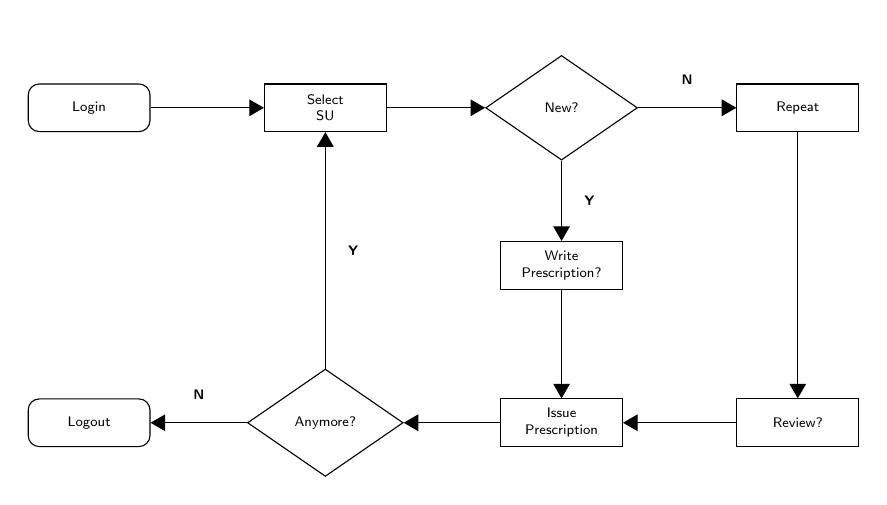
\begin{tikzpicture}
	\node at (0,6) 	[term] (1) {Login};
	\node at (3,6) 	[proc] (2) {Select\\SU};
	\node at (6,6)	[test] (3) {New?};
	\node at (9,6)  [proc] (4) {Repeat};
	\node at (6,4) 	[proc] (5) {Write \\ Prescription?};
	\node at (9,2) 	[proc] (6) {Review?};
	\node at (6,2)	[proc] (7) {Issue \\ Prescription};
	\node at (3,2)  [test] (8) {Anymore?};
	\node at (0,2)  [term] (9) {Logout};

	\node at (6,7)	[zero] (10) {\hfill};
	\node at (0,5)	[zero] (11) {\hfill};

	\draw[solid,->,>=triangle 60]	(1) -- (2);
	\draw[solid,->,>=triangle 60]	(2) -- (3);
	\draw[solid,->,>=triangle 60]	(3) -- (4);
	\draw[solid,->,>=triangle 60]	(4) -- (6);
	\draw[solid,->,>=triangle 60] 	(5) -- (7);
	\draw[solid,->,>=triangle 60]	(6) -- (7);
	\draw[solid,->,>=triangle 60]	(7) -- (8);
	\draw[solid,->,>=triangle 60] 	(8) -- (9);
	\draw[solid,->,>=triangle 60]	(3) -- (5);
	\draw[solid,->,>=triangle 60]	(8) -- (2);

	\path(3) to node[plainLabel,above]{N} (4);
	\path(3) to node[plainLabel,right]{Y} (5);
	\path(8) to node[plainLabel,right]{Y} (2);
	\path(8) to node[plainLabel,above]{N} (9);


\end{tikzpicture}
	\caption{Flowchart for completion of prescription. Note, the scope of this application is not to implement the prescription processes and procedures and therefore simplified. Abbreviation: SU\---Service User.} 
	\label{fig:fc:prescription}
\end{figure}


\subsection{Management}
There are many managerial tasks that could be included here, two were chosen to demonstrate that permissioned blockchain has the capabilities to facilitate such tasks. Two tasks were chosen and discussed below.

\subsubsection{Assign Key worker}
Whilst outside the scope of this prototype, it is recognised that key workers are assigned to service users and have important responsibilities. Assigning a key worker is a managerial duty and is demonstrated here to show how blockchain applications can accommodate such processes as a transaction.


The procedure is simple and shown in fig. \ref{fig:fc:assign}, only a manager can have access to the transaction to assign a healthcare professional as a key worker to a service user (patient). Whilst comparisons can be made to databases, blockchain applications are different and checks should be completed to ensure that both the service user and healthcare professional exist. Once the necessary checks are completed the assignment of the key worker is complete and the manager can log out, or assign another key worker.

Each of these assignments is included on the blockchain, this includes the date, time, manager, service-user and healthcare professional. 
\begin{figure}
\centering
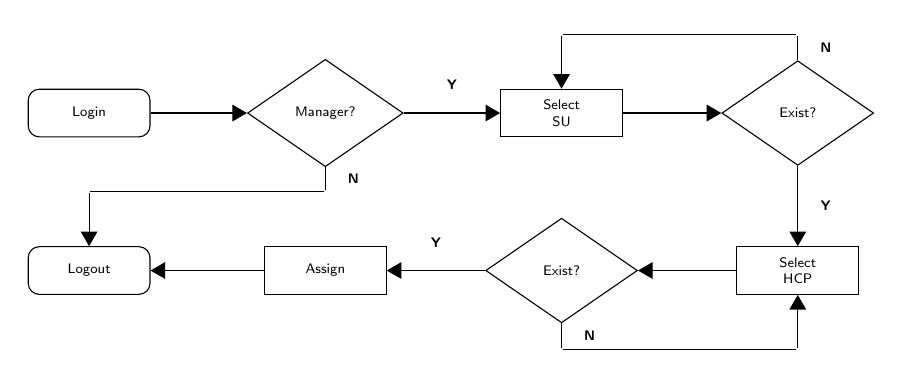
\begin{tikzpicture}
	\node at (0,6) 	[term] (1) {Login};
	\node at (3,6)  [test] (2) {Manager?};
	\node at (6,6) 	[proc] (3) {Select \\SU};
	\node at (9,6)	[test] (4) {Exist?};
	\node at (9,4)	[proc] (5) {Select \\HCP};
	\node at (6,4)  [test] (6) {Exist?};
	\node at (3,4)  [proc] (7) {Assign};
	\node at (0,4)  [term] (8) {Logout};

	\node at (3,5)	[zero] (10) {\hfill};
	\node at (0,5)	[zero] (11) {\hfill};
	\node at (9,7) 	[zero] (12) {\hfill};
	\node at (6,7)	[zero] (13) {\hfill};
	\node at (6,3)	[zero] (14) {\hfill};
	\node at (9,3)	[zero] (15) {\hfill};

	\draw[solid,->,>=triangle 60]	(1) -- (2);
	\draw[solid,->,>=triangle 60]	(2) -- (3);
	\draw[solid,->,>=triangle 60]	(3) -- (4);
	\draw[solid,->,>=triangle 60]	(4) -- (5);
	\draw[solid,->,>=triangle 60] 	(5) -- (6);
	\draw[solid,->,>=triangle 60]	(6) -- (7);
	\draw[solid,->,>=triangle 60]	(7) -- (8);

	\draw[solid]	(2)--(10);
	\draw[solid]	(10)--(11);
	\draw[solid,->,>=triangle 60]	(11) -- (8);
	\draw[solid]	(4)--(12);
	\draw[solid]	(12)--(13);
	\draw[solid,->,>=triangle 60]	(13) -- (3);
	\draw[solid]	(6)--(14);
	\draw[solid]	(14)--(15);
	\draw[solid,->,>=triangle 60]	(15) -- (5);

	\path(2) to node[plainLabel,above]{Y} (3);
	\path(2) to node[plainLabel,right]{N} (10);
	\path(4) to node[plainLabel,right]{Y} (5);
	\path(4) to node[plainLabel,right]{N} (12);
	\path(6) to node[plainLabel,above]{Y} (7);
	\path(6) to node[plainLabel,right]{N} (14);


\end{tikzpicture}
	\caption{Flowchart for completion of assigning keyworker to service-user (Patient). Abbreviations: SU\---Service User; and, HCP\---Healthcare Professional.}
	\label{fig:fc:assign}
\end{figure}


\subsubsection{Register Service-User with Home}
The flowchart in fig. \ref{fig:fc:register} illustrates the process of registering a service user with a healthcare provider. The issue here is one of access control and cannot be shown on a simplified flowchart, as soon as the service-user is registered, the access control to their records changes. The healthcare provider they were moving from relinquishes access control to the individual's records, whilst the healthcare provider they are moving to gains access control to the individual's records. 

A central authority issues the approval, in the case where the service user is moving between different healthcare providers this could be an NHS Trust or GP. In the case where the service user is moving to a different residence owned by the same healthcare provider, this authority would come from the area manager for that organisation. 

The smart contract would be enacted when the move of the service user has been approved. Using ABAC \cite{nist:abac2014}, which is support by Hyperledger Fabric, the access control is changed on the attributes of the participants and assets, so the implementation is seamless and requires no further work. For example, the healthcare professional administrating medication requires access to the service user's records, for this the healthcare professional needs the required attributes to have `READ' access to these records. Put simply, the residence would have to be equal for both the service user and the healthcare professional, further attributes can be added, such as the healthcare professional has to be registered, qualified and if there is a system to clock-in then confirmed that he or she is on-site. Hyperledger's Access Control Language (ACL) can easily implement such conditions and ensure that confidentiality is not breached. 

Two additional systems have been introduced here, a central authority to approve the move of the service user, and a system to monitor employees when they are present at the residence (all visitors and employees have to register when they are enter and leave the premises). Permissioned blockchain can easily allow additional authenticated users with limited access control, even of a non-person entity (NPE) variety, as in the case of a clock-in system. 


\begin{figure}
\centering
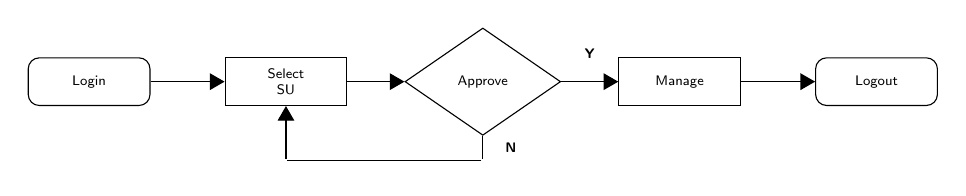
\begin{tikzpicture}
	\node at (0,6) 		[term] 	(1) 	{Login};
	\node at (2.5,6) 	[proc]	(2)	{Select \\ SU};
	\node at (5,6)		[test]	(3)	{Approve};
	\node at (7.5, 6)	[proc]	(4)	{Manage};
	\node at (10,6)		[term]	(5)	{Logout};

	\node at (5,5)		[zero]	(10)	{\hfill};
	\node at (2.5,5)	[zero]	(11)	{\hfill};

	\draw[solid,->,>=triangle 60]	(1) -- (2);
	\draw[solid,->,>=triangle 60]	(2) -- (3);
	\draw[solid,->,>=triangle 60]	(3) -- (4);
	\draw[solid,->,>=triangle 60]	(4) -- (5);

	\draw[solid] 	(3)--(10);
	\draw[solid]	(10)--(11);
	\draw[solid,->,>=triangle 60]	(11) -- (2);

	\path(3) to node[plainLabel,right]{N} (10);
	\path(3) to node[plainLabel,above]{Y} (4);

\end{tikzpicture}
	\caption{Flowchart for registering a Service-User with a Healthcare provider. Abbreviations: SU\---Service User.}
\label{fig:fc:register}
\end{figure}

\subsection{Medical Administration}
Completion of the Medical Administration Records Sheet is an important task for the welfare of the service-user. BMAR does not make any claims that it improves this procedure, merely that it can be implemented and all actions recorded without modification. In fact, caution should be taken if this was implemented since there are effects of introducing automated systems, e.g., post-completion error, whereby the appropriately qualified Healthcare Professional completes the form, but forgets to complete the task and administer the medication, see \cite{li2005post} for further information.

Whilst caution and further research should be taken, there is evidence that the \cite{bennett2003computerised,bates1998effect}, that medication administration could benefit from the introduction of such technologies. 

\begin{figure}
\centering
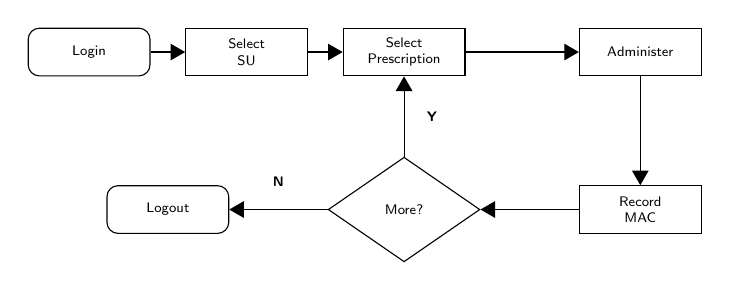
\begin{tikzpicture}
	\node at (0,6) 	[term] (1) {Login};
	\node at (2,6) 	[proc] (2) {Select \\SU};
	\node at (4,6)	[proc] (3) {Select \\Prescription};
	\node at (7,6)	[proc] (4) {Administer};
	\node at (7,4)  [proc] (5) {Record \\ MAC};
	\node at (4,4)  [test] (6) {More?};
	\node at (1,4)  [term] (7) {Logout};

	\draw[solid,->,>=triangle 60]	(1) -- (2);
	\draw[solid,->,>=triangle 60]	(2) -- (3);
	\draw[solid,->,>=triangle 60]	(3) -- (4);
	\draw[solid,->,>=triangle 60]	(4) -- (5);
	\draw[solid,->,>=triangle 60] 	(5) -- (6);
	\draw[solid,->,>=triangle 60]	(6) -- (7);
	\draw[solid,->,>=triangle 60] 	(6) -- (3);

	\path(6) to node[plainLabel,right]{Y} (3);
	\path(6) to node[plainLabel,above]{N} (7);

  
\end{tikzpicture}
	\caption{Flowchart for completion of MAR sheet. Abbreviations: SU \--- Service User; and, MAC \--- Medication Administer Code, can be values such as taken, refused, vomit, sleeping or absent.}
	\label{fig:fc:mar}
\end{figure}


\subsection{Medical Observation}
As expected the process for observation of medication is similar to the administration of medication and is shown in fig. \ref{fig:fc:observation}. This process is mandatory for all controlled drugs. After logging-in the observer selects the correct service user and associated prescription, and this would be completed in parallel with the person administrating the medication. Once the medication has been administered the observer enters the correct MAC. If there are multiple prescriptions then the process is repeated.

There are some anomalies that the audit can reveal, for example when an observation is recorded as a transaction on the blockchain before the administration. This, and other queries are discussed in secti\ref{sec:audits} on audits.


\begin{figure}
\centering
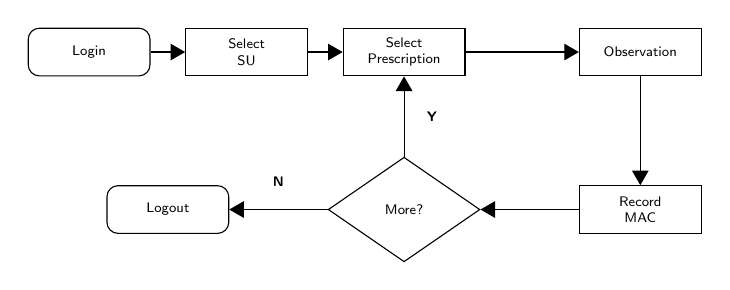
\begin{tikzpicture}
	\node at (0,6) 	[term] (1) {Login};
	\node at (2,6) 	[proc] (2) {Select \\SU};
	\node at (4,6)	[proc] (3) {Select \\Prescription};
	\node at (7,6)	[proc] (4) {Observation};
	\node at (7,4)  [proc] (5) {Record \\ MAC};
	\node at (4,4)  [test] (6) {More?};
	\node at (1,4)  [term] (7) {Logout};

	\draw[solid,->,>=triangle 60]	(1) -- (2);
	\draw[solid,->,>=triangle 60]	(2) -- (3);
	\draw[solid,->,>=triangle 60]	(3) -- (4);
	\draw[solid,->,>=triangle 60]	(4) -- (5);
	\draw[solid,->,>=triangle 60] 	(5) -- (6);
	\draw[solid,->,>=triangle 60]	(6) -- (7);
	\draw[solid,->,>=triangle 60] 	(6) -- (3);

	\path(6) to node[plainLabel,right]{Y} (3);
	\path(6) to node[plainLabel,above]{N} (7);

  
\end{tikzpicture}
	\caption{Flowchart for completion of observation for MAR sheet. Abbreviations: SU \--- Service User; and, MAC \--- Medication Administer Code, can be values such as taken, refused, vomit, sleeping or absent.}
	\label{fig:fc:observation}
\end{figure}


\subsection{Audit and security}\label{sec:audits}
An audit agency, such as the Care Quality Commission, would have `READ' access to all records and transactions on the system. Predefined queries can be completed for each healthcare provider, grouped by residence and service user. Often the accumulation of these reports makes it difficult to find anomalies, however, search algorithms can be deployed and queries can be designed to find any issues that may arise. For example, a MAR sheet error can be self-audited and left to the expertise of the auditor to question the manager of the care home. This is nothing new, however, the innovative part is the use of blockchain technologies to ensure a disintermediatory append-only ledger of MAR sheets, which makes it impossible to retrospectively delete or correct. There are arguments about a 51\% attacks \cite{bastiaan2015preventing}, which are theoretical and often discussed with permissionless blockchain technology. Firstly, with permissioned blockchain, the likelihood of such an attack is diminished further since all nodes in the network are authenticated by an access control layer. Secondly, such an attack would require changing more than $\frac{2}{3}$ of nodes since the consensus algorithm, PBFT \cite{castro1999practical}, used requires a higher percentage of agreement. 
This vulnerability of permissioned blockchain has an extremely low probability of success, nevertheless, it is mathematically possible and discussed in \cite{zyskind2015decentralizing}. The transaction process is fully encrypted and Hyperledger Fabric requires participants to be certified and therefore providing a security infrastructure for authorisation and authentication, see \cite{cachin2016architecture} for more details. 


%And thirdly, on permissioned blockchains there is a low-latency high transaction throughput, this means that from the genesis block a high number of transactions per second (TPS), this would have to be halted in order to complete the attack. Yes, this is a vulnerbility but one that can be monitored. 
%The next issue of security is device breach. In the results only the logical system was tried and tested, however, the physical system would require handheld digital devices for healthcare professionals to complete MAR transactions. Furthermore access to the blockchain from other devices is required, e.g. managers and auditors, so device breach is an issue for any system. Do not confuse permissionless with permissioned blockchain, permissionless blockchains verify transactions and broadcast them over a network, in which anyone can join. 



\section{Results}\label{sec:results}
The access latency for transactions is instantaneous, for BMAR there are relatively small amounts of data, $<$1Kbyte, uploaded to the permissioned blockchain and the delay is negligent. Hyperledger has demonstrated elsewhere with documents ($>$10Kbyte) the access latency is less than 2 seconds \cite{androulaki2018hyperledger}. The latency has not been fully tested, however, other implementations \cite{thakkar2018performance} indicate that access latency is dependent on transactions per second and block size. 

The tests were mainly completed to see how the blockchain could be accessed and processed by key personnel involved in the care and support of a service-user. The development and implementation gave a valuable and insightful understanding of the nuances of administration of medication process. The decision to separate data was based on some rationale regarding access to data, e.g. should auditors be able to identify a service-user or healthcare professional by name? Is there a need for an auditor, when the system can audit itself? These questions are visited in the conclusions. The data stored in asset and participant registries has restricted access. 

\subsection{Prescription}
The prescription process has been simplified, but it is possible that the details provided below can be provided from other systems used by the healthcare profession. The prescription process is outside the scope of this project, and essentially the list of information provided in fig. \ref{fig:lst:prescription} is minimal requirement. The information can only be provided by a qualified GP or equivalent, and `READ' access is given to other participants in the system. The transaction records the date and the participant who issued the prescription (not shown). A quick breakdown of the code in fig. \ref{fig:lst:prescription} shows on line 4 a unique identifier for the prescription, line 5 the unique identifier for the service user, line 6 the unique identifier of the medication and lines 7\--14 the details of the prescription. 
\begin{figure}
	\tiny
	\begin{lstlisting}[language=json,firstnumber=1]
=========== REGSITRY ============
{
  "$class": "org.bmar.net.Prescription",
  "ID": "5579",
  "Patient": "resource:org.bmar.net.SU#S111",
  "PrescribedMedication": "resource:org.bmar.net.Medication#111",
  "initialisation": "2018-10-25T17:26:56.674Z",
  "Form": "Pill",
  "Route": "Oral",
  "Controlled": false,
  "Duration": "4",
  "Dose": "25",
  "Quantity": 1,
  "Instructions": "One (1) tablet two (2) times a day"
}
=========== TRANSACTION =============
{
 "$class": "org.bmar.net.Prescribe",
 "actualPrescription": "resource:org.bmar.net.Prescription#5579",
 "transactionId": "91a39021-d1b7-4c8e-9eb2-540b82e641fe",
 "timestamp": "2018-10-25T17:30:29.706Z"
}
	\end{lstlisting}
	\caption{Transaction for Prescription, output shows entry for a prescription in the asset registry, `Prescription'.}
\label{fig:lst:prescription}
\end{figure}


\subsection{Medical Administration}
Records in the registry can be altered, every update of the records in the registry is written to the blockchain. So, all changes to assets and participants are recorded on the blockchain in perpetuity. Medical Administration is no exception and is conducive to blockchain technology due to its auditable nature.  

Lines 1\--32 in fig. \ref{fig:lst:administration} shows the result of a change in the records for an administration of a prescription, `5579', to a service-user, `S111', at a Healthcare Provider, `H1'. Line 29 indicates that actual medication administration code (MAC) recorded by the Healthcare professional was `taken'. Line 30 indicates that this was not confirmed by the observer, which is completed by a different transaction and updated accordingly. 

There are some important omissions of information that are required. This vital information is stored in the associated transaction display between lines 34\--42. Here the relationship to the service user is stored, `S111' (line 36), the prescription, `5579', the timestamp and finally, the transaction ID. The healthcare professional completing the medication administration is recorded as access on the blockchain, not shown here. 


\begin{figure}
	\tiny
	\begin{lstlisting}[language=json,firstnumber=1]
=========== REGSITRY =============
{
  "$class": "org.bmar.net.MAR",
  "time": "1540490058276",
  "actualPrescribedMed": {
    "$class": "org.bmar.net.Prescription",
    "ID": "5579",
    "Patient": "resource:org.bmar.net.SU#S111",
    "PrescribedMedication": "resource:org.bmar.net.Medication#111",
    "initialisation": "2018-10-25T17:26:56.674Z",
    "Form": "Pill",
    "Route": "Oral",
    "Controlled": false,
    "Duration": "4",
    "Dose": "25",
    "Quantity": 1,
    "Interval": 0,
    "Instructions": "One (1) tablet two (2) times a day"
  },
  "actualPatient": {
    "$class": "org.bmar.net.SU",
    "ID": "S111",
    "firstName": "S",
    "lastName": "U",
    "Allergies": "none",
    "DoB": "1991-08-10T00:00:00.000Z",
    "KeyWorker": "resource:org.bmar.net.HCP#HP111",
    "Home": "resource:org.bmar.net.HealthCareProvider#H1"
  },
  "actualMAC": "taken",
  "ObservedMAC": "unconfirmed"
}
=========== TRANSACTION ============= 
{
 "$class": "org.bmar.net.Administer",
 "Patient": "resource:org.bmar.net.SU#S111",
 "actualPrescribedMed": "resource:org.bmar.net.Prescription#5579",
 "time": "2018-10-25T20:02:29.832Z",
 "recordedMAC": "taken",
 "transactionId": "7d919a4c-2c71-4ea6-a073-deffb3e19fc3",
 "timestamp": "2018-10-25T20:03:15.236Z"
}
	\end{lstlisting}
\caption{Ouput for transaction for Administration. Top half is stored on registry, the bottom half is stored on blockchain.}
\label{fig:lst:administration}
\end{figure}

\begin{figure}
	\tiny
	\begin{lstlisting}[language=json,firstnumber=1]
=========== REGSITRY ============= 
{
  "$class": "org.bmar.net.MAR",
  "time": "1540490058276",
  "actualPrescribedMed": {
	  ............
    },
  "actualPatient": {
	  ............
  },
  "actualMAC": "taken",
  "ObservedMAC": "taken"
}
=========== TRANSACTION =============
{
 "$class": "org.bmar.net.Observe",
 "unconfirmedMAR": "1540490058276",
 "ObservedMAC": "taken",
 "transactionId": "22b1d98c-70e2-46c6-83a2-9637ad36698e",
 "timestamp": "2018-10-25T20:25:02.478Z"
}
\end{lstlisting}
	\caption{Ouput for transaction for Observation. For brevity, the information in the `actualPrescribedMed' and `actualPatient' are not displayed here and are the same as in fig. \ref{fig:lst:prescription}.}
\label{fig:lst:observation}
\end{figure}

\subsection{Observation}
Lines 2\--13 in fig. \ref{fig:lst:observation} shows the changes to the asset as a result of the observation transaction. Lines 6 and 9 are the same information as the information stored in the administration transaction in fig. \ref{fig:lst:administration} and for brevity not repeated here.  On line 11 the recorded MAC is entered as `taken' as entered in a previous transaction. The important change is to compare lines 31 and 12 in fig. \ref{fig:lst:administration} and \ref{fig:lst:observation}, respectively. The value assigned to the attribute, `{\tt ObservedMAC}' has changed from `{\tt unconfirmed}' to `{\tt confirmed}', which matches the value in the transaction (line 18 in fig. \ref{fig:lst:observation}. In the transaction, the timestamp is recorded at, `2018-10-25T20:25:02.478Z', some 22 minutes are the administration of the medication. 

The ID of the individual MAR was completed as converting a timestamp to a string, in fact on line 4 in fig. \ref{fig:lst:observation} the asset attribute name is `{\tt time}'. In a system where there are potentially millions of MAR entries, this could be a little simplistic, although it works for our prototype. In such situations, Hyperledger suggests to merge and split attributes to maintain their unique identity, so an obvious candidate is the prescription ID.

Finally, not shown in the transaction is the identity of the healthcare professional conducting the observation, this is included on the blockchain and not shown here.


\section{Management}
Access to management functions would be restricted to Managers and entirely role-based. However, there are the attributes of the asset or participant being managed to take into consideration. These two options demonstrate the participant management.

Lines 2\--11 in fig. \ref{fig:lst:management} shows the data stored in the blockchain as a result of the transaction.
The service user, identified as `S444' (line 4), has been assigned a key worker `HP333' (line 9) and registered at a healthcare provider, identified as `H1' (line 10). 

The transaction of the service user to the healthcare provider is shown in lines 13\--18 in fig. \ref{fig:lst:observation}. An existing service user and home have been selected. The transaction timestamp is on line 17 and should pre-date the following transaction.

The transaction of assigning a key worker to the service user is shown in lines 20\--26 in fig. \ref{fig:lst:observation}. The pre-conditions for this is that the service user selected has to be registered to a healthcare provider managed by the manager completing the transaction, and the key worker is a healthcare professional working at the same healthcare provider. The transaction timestamp is on line 25 and post-dates registering a service user with a healthcare provider. 



\begin{figure}
\tiny
	\begin{lstlisting}[language=json,firstnumber=1]
===========REGISTRY=============
{
  "$class": "org.bmar.net.SU",
  "ID": "S444",
  "firstName": "B",
  "lastName": "C",
  "Allergies": "",
  "DoB": "1994-07-25T00:00:00.000Z",
  "KeyWorker": "resource:org.bmar.net.HCP#HP333",
  "Home": "resource:org.bmar.net.HealthCareProvider#H1"
}
===========REGISTER SU TRANSACTION=============
{
 "$class": "org.bmar.net.RegisterSU",
 "Patient": "resource:org.bmar.net.SU#S444",
 "Home": "resource:org.bmar.net.HealthCareProvider#H1",
 "transactionId": "4b25df90-5dec-47e0-b58d-511908225343",
 "timestamp": "2018-11-01T13:29:07.629Z"
}
===========ASSIGN KEYWORKER TRANSACTION=============
{
 "$class": "org.bmar.net.assignKeyWorker",
 "newKeyWorker": "resource:org.bmar.net.HCP#HP333",
 "Patient": "resource:org.bmar.net.SU#S444",
 "transactionId": "e2d55441-813e-4785-8e6c-04b44bca5818",
 "timestamp": "2018-11-01T13:31:16.812Z"
}
	\end{lstlisting}
\caption{Output for management transactions. Registry shows data held on particpant after two transactions completed below.}
\label{fig:lst:management}
\end{figure}

\begin{figure}
	\centering
	\includegraphics[scale=.50]{audit2.png}
	\caption{Audit view for transactions}
	\label{fig:audit}
\end{figure}

\subsection{Audit}
Various queries can be set up to produce reports for auditors. Fig. \ref{fig:audit} illustrates one of many views an auditor may have, here is a sample of the transactions made for management. The key problem in the above examples is seeing who completed the transactions, here by simply matching the timestamps reveals who submitted the transaction:
\begin{description}
	\item[2018-11-01T13:29:07.629Z:] Matching this transaction from fig. \ref{fig:lst:management} (line 18) to fig. \ref{fig:audit} shows that the transaction was to `RegisterSU' and conducted by `M111(Manager)'.
	\item[2018-11-01T13:31:16.812Z:] Matching this transaction from fig. \ref{fig:lst:management} (line 26) to fig. \ref{fig:audit} shows that the transaction was to `assignKeyWorker' and conducted by `M111(Manager)'.
\end{description}



\section{Conclusions}
\label{sec:conclusions}

There are many proposed blockchain healthcare systems, e.g., see \cite{zhang2017applying,griggs2018healthcare,azaria2016medrec,vithanwattana2017developing}. However, whilst these proposed systems are all meaningful, the prototype for BMAR is for a different application and designed for the recording and auditing of medication administration records. 

All Caldicott principles have been considered in the design of this application and meaningful-use would be the reduction of MAR sheet errors with the overall intention of improving health services and safeguarding vulnerable adults. The permissioned blockchain application provides the security and privacy required for health informatics. The data is permanent and immutable, which makes it an ideal technical solution to the MAR sheet problem.
 

During the design and implementation stages, it was considered that much of the data will already be available as EHR. It is highly likely that such an implementation would require the use of EHR in an existing database and therefore it is recommended to keep registries relatively static since it is the transactions that change. Such designs lead to keeping databases relatively static and a reliance on blockchain for transactions and change. As a recommendation, when designing a blockchain application it is useful to identify transactions. As yet, there is no standard modelling technique for blockchain and therefore remains a  challenge in designing applications. It is recommended that robust modelling techniques are required for building blockchain applications, especially for the modelling and differentiation between transactional, asset and participant data.  

From the prototype of BMAR the benefits of using blockchain to manage EHR are as follows: 

\begin{itemize}
	\item {\bf Disintermediation} is often referred to as the 'removal of the middleman' \cite[ch. 1]{hyperledger:gaur2018}. One of the many promises of permissionless blockchain is the to complete financial transactions without the need of a central banking authority. Permissioned blockchain is no exception and aims to reduce the number of intermediaries between producer and consumer. Whilst BMAR may not have many intermediaries, the process of integration of existing services does not pose a problem. 
 	\item{\bf Prevention} and reduction of medication administration errors. Further research would be required for evidence that BMAR would reduce medication administration errors, however, similar studies \cite{bates1998effect,bennett2003computerised} give supporting evidence that medication administration errors can be reduced by the introduction of automated systems. The prevention would come in the form of sending reminders to appropriate healthcare professionals that an administration of medication is due. 
	\item {\bf Integrity} of EHR. BMAR requires generates a report of MAR sheets, inspected by quality assurance agencies (e.g. CQC) and produced by a healthcare agency. Normally, the inspection would be completed by paper and there would be an issue of trust. Unlikely as it is, physical MAR sheets are designed as append-only, which is why permissioned blockchain are so apt as a technological solution. However, there is only one MAR sheet that normally covers a week for each service-user, and it is not inconceivable for this paperwork to be exposed to the temptation to adjust or rewrite them given the correct circumstances. There has to be an element of trust between the auditor and the healthcare provider to assess the integrity of the information provided. With permissioned blockchain, even given the correct circumstances the ability to make any amendments to the form retrospectively is virtually impossible. The integrity of the EHR generated by BMAR is to be trusted by all parties.
	\item{\bf Cost} in Health Information Technology (HIT) has mixed reviews, with many claiming the high costs and investment \cite{adler2011survey} in healthcare systems simply do not deliver. This is often referred to as the productivity paradox \cite{bui2018cacm}. Nevertheless, there are examples of closed studies that report immediate benefits of HIT \cite{bennett2003computerised,bates1998effect}. BMAR is to implement a prototype for a blockchain application for MAR sheets and report on self-auditing and reminders sent to assigned staff. 
	\item {\bf Interdependency} between agencies in the healthcare sector is high. At its best, this can affect cost, with duplicate tests for patients issued by different physicians due to `information blocking', whereby physicians do not have sufficient privileges to access data from other organisations \cite{azaria2016medrec}. At its worse provide opportunities for rogue physicians to exploit the system. Even for the production of MAR sheets, there is some interdependency between healthcare provider, primary carer and auditors, see principle 7 of Caldicott. Blockchain not only provides a technical solution but in addition provides a system whereby the other interdependent agencies can trust each other's information.
	\item{\bf Security and Integrity} of personal data. In BMAR there is pseudo-anonymous data stored in transactions, and personal and confidential data about service users stored in the registries. With de-anonymity algorithms, e.g., \cite{de2013unique}, and enough reference points pseudo-anonymised data can easily be used to identify individuals. All data needs protection and permissioned blockchain provides the security and ensures the integrity of the data, see \cite[ch. 5]{gupta:2018} for further details.
	\item{\bf Auditability} of MAR sheets. Blockchain provides transparent governance and/or auditing. Viewing information in reports generated by a system can be difficult to search. BMAR can assist this since it has the information when medication is to be administered and to who. Therefore, it can self-regulate and highlight errors, essentially highlight errors after reminders have been sent. The auditing agency can review the generated reports at any time and then look into further details as to why there are MAR errors. BMAR is not going to replace the expertise of the individuals but simply give individuals the information required to complete an inspection. 
\end{itemize}

The prototype for BMAR requires further research and development, however, for the reasons above the introduction of such a system would benefit healthcare professionals, healthcare providers and service users. 

\subsubsection*{Competing Interests}
None identified.

\subsubsection*{Acknowledgements} The authors would like to thank the invaluable information gain from interviewing healthcare professionals in the design and implementation of BMAR.

\bibliographystyle{plain}
\bibliography{../forensic2}


\end{document}
